\chapter{Travaux réalisés}

\section{Séparation des tâches}
\paragraph{}
Nous constatons assez rapidement dans le projet qu'il est très difficile d'utiliser
le SDK de la Kinect et la DLL directement dans Unity. Plusieurs projets, trouvé durant nos recherches, utilisent un système 
de socket afin de pouvoir envoyer des informations à une application Unity3D à partir d'une application C\#.
Nous utilisons donc la même méthode afin de pouvoir séparer les différentes tâches de notre projet.

\paragraph{}
Nous créons donc un client utilisant la DLL et qui effectue l'ensemble des opérations sur les données afin
de les envoyer à une application Unity3D qui n'a plus qu'à effectuer les transformations sur le modèle avec
les données reçu. En effet, les données fournis pas la DLL ne peuvent être appliqué tel quel sur le modèle.
Le repère des coordonnées fournis par la DLL est le repère image, donc un repère en 2D en pixel. Or, notre 
application doit modèliser la main dans un environnement 3D.

% \paragraph{}
% Pour avoir une animation de la main la plus précise possible, nous récupérons également les points fournis par
% le SDK de la Kinect pour avoir plus d'information, mais également de vérifier les résultats calculés par 
% la DLL. Cette vérification ce fait sur le bout du pousse et sur le bout du majeur, car ces points sont communs
% à la DLL et au SDK.

\begin{figure}[H]
  \label{carte_main}
  \begin{center}
    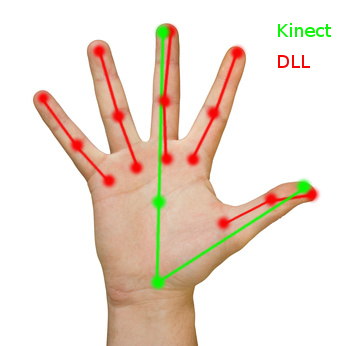
\includegraphics[width=200px]{images/main2.png}
    \caption{Carte des points de la main détectés par la DLL et la Kinect}
  \end{center}
\end{figure}

\paragraph{}
L'intérêt de cette séparation est que notre méthode de localisation des jointures se repose sur une 
DLL et que les calculs effectués sur les données sont spécifiques a celle-ci. En cas de changement de 
technologie, il suffit de modifier le client sans avoir à changer l'application Unity3D. La seul contrainte
étant la structure des socket envoyé. Nous avons donc une application modulable permettant de modifier 
facilement la méthode de récupération des jointures, mais aussi de modifier le matériel utilisé.

\begin{figure}[H]
  \label{schema_application}
  \begin{center}
    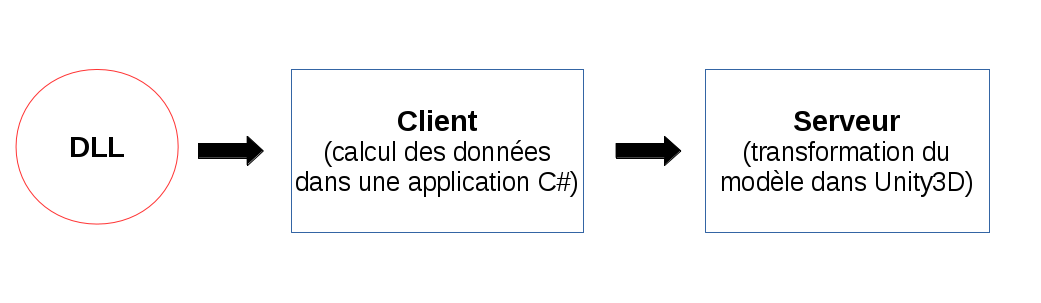
\includegraphics[width=350px]{images/schemaAppli.png}
    \caption{Schéma de la structure de l'application}
  \end{center}
\end{figure}

%TODO La traduction de "joint" est "articulation" en français, dans notre cas.
% Comme jointure est un peu partout dans le rapport je pense qu'on va le laisser. 
\section{Récupération de la position des articulations de la main}
\label{Real_get_art}
\paragraph{}
Le premier problème à résoudre est donc le calcul de la troisième coordonnée de chaque jointure. Grâce à la Kinect,
il est possible de récupérer les coordonnées, dans le repère monde, de la jointure du poignet. Elle nous permet
également de récupérer une valeur dans l'image de profondeur, valeur représentant la troisième coordonné d'un point.
Nous avons alors la valeur du pixel de l'image de profondeur de la jointure recherché $p_{recherche}$, la valeur
du pixel de l'image de profondeur de la jointure du poignet $p_{ref}$ et la valeur de la troisième coordonné dans 
le repère monde de la jointure du poignet $z_{ref}$. Nous appliquons alors une règle de trois pour obtenir 
la valeur dans le repère monde de la troisième coordonné de la jointure courante.

\begin{equation}
 z_{recherche} = \frac{z_{ref} * p_{recherche}}{p_{ref}}
\end{equation}

\paragraph{}
La seconde problématique de notre méthode est la normalisation des coordonnées que nous avons récupérer. Les coordonnées
de la kinect sont dans le repère monde, nous avons donc besoin d'utiliser les caractéristiques de la caméra pour normaliser
les coordonnées. Nous prenons une distance de 4m pour la profondeur de la caméra, car cela correspond à la zone de détection de
la Kinect (voir Fig. \ref{fig:kinect1vs2}).

\paragraph{}
%TODO elliot : revoir paragraphe
%TODO les angles se font coté unity maintenant
Enfin la dernière problématique est de mettre en correspondance les points calculés dans la partie client avec les points du modèle de la partie serveur. Cette mise en correspondance ce fera coté serveur et sera expliqué dans la partie \og modélisation et animation de la main \fg de ce rapport (\textit{cf.} \ref{Real_Animation}).

%mettre image blender model + ajouter axe sur image

\section{Structure du message envoyé par sockets}
\paragraph{}
Nous formatons un message contenant les informations de la 
Kinect et les coordonnées des jointures récupérées précedemment. Ce 
message est créé par le client pour être envoyé au serveur via le 
procole UDP. Enfin le message est traité par le serveur, afin d'obtenir 
les données sous forme de variables exploitable.

\paragraph{}
Au cours du projet, les informations transmies au serveur ont évolué. 
Dans un premier temps, nous envoyions un message lorsque la DLL fonctionnait. 
La permier version du message contenait uniquement les coordonnées des 
jointures détectées par la DLL avec leurs coordonnées Z normalisées (voir Fig. \ref{fig:socketv1}).
Ces coordonnées ne sont pas suffisantes pour l'animation complète de la 
main. Par exemple, la position du poignet est requise pour l'animer 
sur Unity.

\begin{figure}[H]
  \label{fig:socketv1}
  \begin{center}
    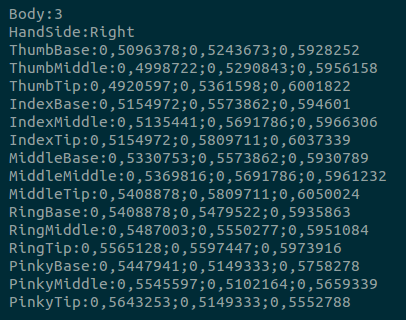
\includegraphics[width=180px]{images/socket_v1.png}
    \caption{Première version du message.}
  \end{center}
\end{figure}

Dans second temps, nous avons ajouté les informations provenant de la 
Kinect en plus de celles de la DLL. Dans ce message nous retrouvons 
les positions relatives au mains calculé par la Kinect. En plus des 
coordonnées des jointure de la DLL nous avons les positions :\\
\begin{itemize}
  \item du poignet
  \item du centre de la main
  \item du bout de la main
  \item du pouce
\end{itemize}
\paragraph{}
Nous transmettons également le status de la main que la Kinect a 
assigné. Le message est envoyé lorsque les status sont \og lasso \fg, \og closed \fg ou 
\og open \fg, (voir Fig. \ref{fig:socketv2}). Pour certaines images 
acquisent par la Kinect, les fonctions de la DLL ne retrouve aucun 
résultats. Par exemple, lorsque l'on ferme la main, la DLL ne détecte 
plus les doigts et aucun message n'est envoyé, alors que la Kinect a 
détecté les points de la main.

\begin{figure}[H]
  \label{fig:socketv2}
  \begin{center}
    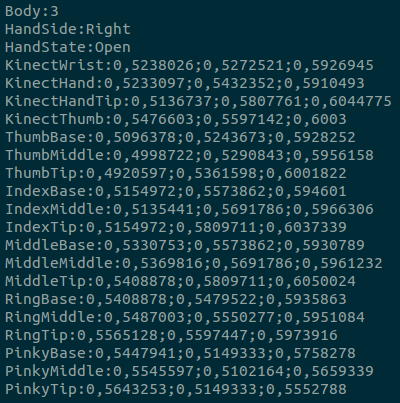
\includegraphics[width=180px]{images/socket_v2.png}
    \caption{Deuxième version du message.}
  \end{center}
\end{figure}

Enfin, nous optons pour deux messages diffèrents. Un message 
est envoyé quand la DLL n'a pas détecté de points. Et un message 
différent est envoyé quand la DLL a retrouvé les jointures de la main (voir Fig. \ref{fig:socketv3}).
Le champ \texttt{AiolosDLLStatus} est ajouté pour différencier les 
messages.

\begin{figure}[H]
  \label{fig:socketv3}
  \begin{center}
    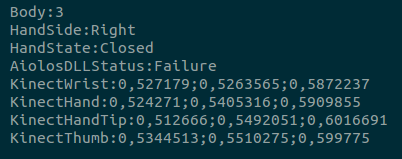
\includegraphics[width=180px]{images/socket_v3-2.png}
    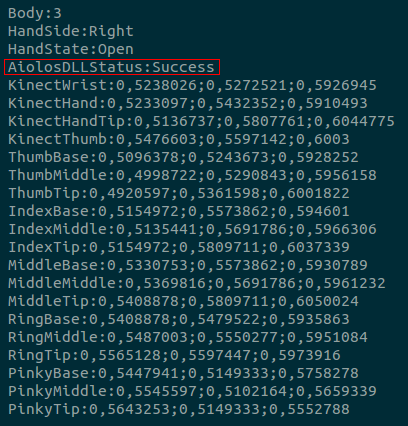
\includegraphics[width=180px]{images/socket_v3-1.png}
    \caption{Versions actuelles des messages. À gauche, DLL non fonctionnelle. À droite, DLL fonctionnelle.}
  \end{center}
\end{figure}


\section{Modélisation et animation de la main}
\label{Real_Animation}
\paragraph{}
%TODO pas besoin de savoir d'ou vient le modele
Nous avons choisi de ne pas modéliser la main de l'utilisateur, à la place, nous avons récupéré un modèle de main existant.
%TODO revoir la tournur de phrase
Sous Blender, nous avons appliqué à ce modèle une armature pour pouvoir l'animer de façon réaliste. Cette armature est constituée d'os et de jointures. L'armature est représenté avec une structure 
d'arbre, avec les noeuds qui représentent les os, et les arcs qui représentent les jointures. Les transformations de chaque fils dépendent des transformations de leurs père. Ainsi, un mouvement du poignet 
entraine le mouvement de chaque os de la main. Cette armature pourra être utilisée pour mimer la main de l'utilisateur. 

\paragraph{}
%TODO ne pas mettre de retourner à l'état de l'art -> peut etre mettre une reference en latex si besoin
Pour relier l'armature au modèle, on utilise une méthode de \og skinning \fg (\textit{cf} \ref{animation}). Dans Blender, on peut utiliser différent types de skinning, 
soit \og à la main \fg \ en créant des groupes de sommets à associer à chaque jointures, soit en utilisant des algorithmes de création des groupes et d'attribution automatique des 
sommets à ces groupes. Nous avons choisi d'utiliser la méthode \og bone heat weighting \fg \cite{baran2007automatic}. 

\paragraph{}
Le modèle et armature ainsi créés sont importés dans Unity3D tout en conservant les associations effectuées par le skinning. 
Ensuite, on teste ce modèle en l'animant à l'aide de rotations des jointures, on peut ainsi faire prendre des poses à la main (voir Fig. \ref{fig:poseMain}). 

\begin{figure}[!h]
	\centering
	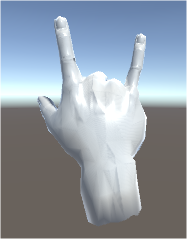
\includegraphics[height=6cm]{images/HandPose1.png}
	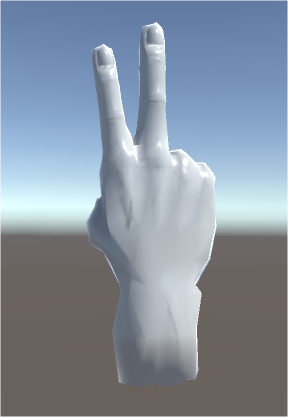
\includegraphics[height=6cm]{images/HandPose2.png}
	\caption{Exemple de poses réalisées à partir de rotations des jointures de l'armature dans Unity}
	\label{fig:poseMain}
\end{figure}

\paragraph{} 
Il existe différentes techniques d'animation basé sur une armature (\textit{cf} \ref{animation}).
Pour notre projet, nous avons choisi la méthode qui utilise les articulations récupérées par la DLL en conjonction avec les points récupérés \textit{via} le SDK de la Kinect. Ces points servent à positionner les jointures de l'armature par translations et/ou rotations.
Cependant, comme expliqué précédemment, il faut mettre en correspondance ces points (\textit{cf.} \ref{Real_get_art}).
Pour cela, le plus simple a été de faire correspondre le point du poignet détecté par la Kinect à la jointure équivalente du modèle.
Cependant, si aucune rotation n'est appliqué sur la main, la position de la base des doigts ne correspond plus et le modèle est déformé voir Fig. \ref{fig:badhand}.
Il faut prendre en compte la rotation du poignet pour que les jointures de l'armature correspondent aux articulations de la main. 
Pour cela, nous gardons en mémoire la rotation du modèle avant l'interaction avec l'utilisateur,
puis nous calculons la rotation à partir de cette angle (\ref{fig:??}). Cette méthode permet de ne pas avoir de modification des axes de rotation suite à une succession de rotation.

%TODO elliot -> explication du calcul de l'angle
% On applique une rotation de l'angle calculé à l'armature du modèle, cela permet de retrouver l'orientation de la main sur l'axe X et Y.
% Une opération similaire est effectuée avec la base du pouce à la place du milieu de la main pour trouver l'orientation en Z: 
%
\paragraph{} 
Une fois le modèle correctement positionné et orienté, il faut s'occuper des doigts.
Nous pouvons voir sur la Fig. \ref{} que le modèle est complètement déformé et ne correspond plus à la main d'un utilisateur. Les points d'un modèle
ne sont pas fait pour être manipulé directement dans l'espace, il est préférable de calculer des angles pour chaque jointure afin de leur appliquer 
des rotations. Une partie complexe a été de décider d'une méthode de calcul des angles des jointures et de l'implémenter.
Nous avons choisi de reprendre la même méthode que pour le poignet en prenant la rotation de départ du modèle et en appliquant une rotation avec le nouvel angle.

\begin{figure}
\label{fig:badhand}
\centering
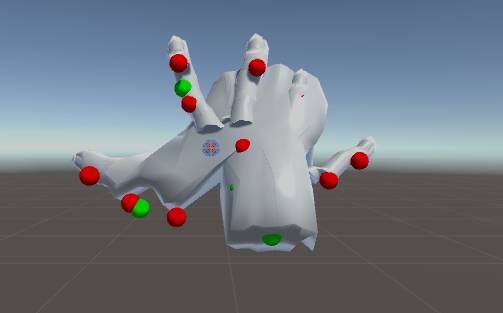
\includegraphics[width=10cm]{images/BadHand.png}
\caption{Exemple de déformation du modèle avant mise en correspondance}	
\end{figure}

%TODO prendre un screenshot de l ecran pour le problème de rotation de la main

%TODO prendre une image de la main avec un axe horizontal et l'angle à calculer
